\documentclass[12pt]{article}
\usepackage{graphicx}
\usepackage[section]{placeins}
\usepackage[italian]{babel}
\usepackage{siunitx}

\graphicspath{{./images/}}

\begin{document}
    \section{Lavoro ed Energia}
    \subsection{Introduzione}
    \paragraph{} L'energia è presente nell'Universo in \textbf{varie forme}. \textbf{Ogni} processo fisico nell'Universo coinvolge \textit{energia e trasferimenti} o \textit{trasformazioni ed energia}.
    \paragraph{} Sfortunatamente, però, essa \textbf{non è facile da definire}.
    \paragraph{} Per parlare di energia occorre definire il concetto di \textbf{sistema} e il concetto di \textbf{ambiente}.

    \subsection{Sistemi e Ambienti}

    \paragraph{} Si definisce \textbf{sistema} un modello secondo il quale la nostra attenzione viene concentrata su una \textbf{piccola regione dell'Universo}, ignorando i dettagli del resto.
    \paragraph{} Occorre quindi \textit{saper identificare il sistema corretto}. Un sistema può:
    \begin{itemize}
        \item Essere un singolo oggetto o particella
        \item Essere un insieme di oggetti o particelle
        \item Essere una regione dello spazio
        \item Variare in dimensioni e forma
    \end{itemize}
    \paragraph{} Si definisce \textbf{contorno del sistema} la superificie \textbf{immaginaria}, che potrebbe anche coincidere con una superificie fisica, che \textbf{divide} il sistema dall'ambiente
    \paragraph{} Si definisce \textbf{ambiente} l'area che agisce sul sistema attraverso il suo contorno
    \newpage
    \subsection{Lavoro}
    \paragraph{} Il \textbf{lavoro} fatto su un sistema da una causa che esercita una forza costante sul sistema è il prodotto del modulo della forza $F$, del modulo dello spostamento $\Delta r$ del punto di applicazione della forza e di $cos \ \theta$, essendo $\theta$ l'angolo compreso tra il vettore forza ed il vettore spostamento.
    $$ W = F \Delta r cos \ \theta$$
    \begin{itemize}
        \item È una \textbf{grandezza scalare}
        \item Il \textbf{segno} dipende dalla direzione di $F$ relativamente a $\Delta r$
        \item L'\textbf{unità di misura è il $J$} [$N \cdot m$]
    \end{itemize}
    \paragraph{} Il lavoro rappresenta un \textbf{trasferimento di energia}
    \begin{itemize}
        \item \textit{dal} sistema se \textbf{negativo}
        \item \textit{al} sistema se \textbf{positivo}
    \end{itemize}
    \paragraph{Lavoro con forza variabile} È la sommatoria di tutte le aree sottese del grafico Forza-spostamento con spostamento infinitesimale
    $$\int_{x_i}^{x_f} F_x \ dx$$
    Se su un sistema agisce \textbf{più di una forza} ed esso \textbf{può essere assimilato ad una particella}, il lavoro compiuto è il lavoro compiuto dalla \textbf{forza risultante}.
\newpage
\subsection{Energia Cinetica}
    Si definisce \textbf{energia cinetica} la forma di energia conseguente ad un \textbf{lavoro compiuto su un sistema}, relativa ad un suo \textbf{cambio di velocità}.
    \paragraph{} Segue l'equazione
    $$W_{est} = {1 \over 2}mv_f^2 - {1 \over 2}mv_i^2$$
    Quest'equazione ci dice che il \textbf{lavoro svolto dalla forza risultante su un particella di massa \textit{m} è uguale alla differenza fra i valori finale e iniziale della grandezza ${1 \over 2}mv^2$}

    \paragraph{} Si deduce quindi che il lavoro compiuto dalla forza risultante è pari alla \textbf{variazione di energia cinetica} della particella
    $$W_{est} = K_f - K_i = \Delta K$$

    \paragraph{} Quest'equazione è nota come \textbf{teorema dell'energia cinetica}, ovvero:
    Quando viene svolto un lavoro su un sistema e la \textbf{sola} variazione nel sistema è il modulo della sua velocità, il lavoro compiuto dalla forza risultante è uguale alla variazione di energia cinetica del sistema\\[12pt]
    \textbf{Dimostrazione:} 
    \begin{figure}[!htb]
        \centering
        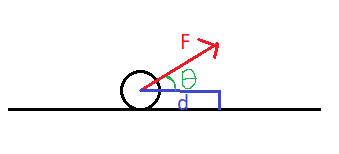
\includegraphics[width=0.35\textwidth]{Lavoro.png}
    \end{figure}
    \begin{itemize}
        \item Trovo $F_x = F \cdot cos \ \theta = ma_x$
        \item Se $F_x$ è \textbf{constante} anche $a$ lo è, quindi posso ricavare la velocità da ${v_f^2 = v_i^2 + 2ad} \rightarrow {a = {{v_f^2-v_i^2} \over 2d}}$
        \item Sostituendo $a_x$ ottengo $F_x = m{{v_f^2-v_i^2}\over 2d}$
        \item $F_xd = {1 \over 2}mv_f^2 - {1 \over 2}mv_i^2 = \Delta K$
    \end{itemize}
    \newpage
    \subsection{Lavoro della forza gravitazionale}
    La forza di gravità 
    \begin{itemize}
        \item Esegue lavoro \textbf{resistente} quando il corpo sale
        \item Esegue lavoro \textbf{a favore} quando il corpo scende
    \end{itemize}
    Applicando il teorema dell'energia cinetica si ha:
    \begin{itemize}
        \item $\Delta K = K_f - K_i = L_f + L_g$
        \item Se $K_f = K_i$ allora si ha che $\Delta K = 0 = L_f + L_g$
        \item Quindi $L_f = -L_g$
    \end{itemize}
    Ovvero \textbf{la forza di gravità toglie tanta energia quanta ne ha fornita $F$ per far salire il corpo}
    \newpage
    \subsection{Lavoro svolto da una molla} Legge di Hook:
    $$F_m = -kx$$
    dove $x$ è la posizione del blocco rispetto all'equilibrio
    \begin{itemize}
        \item Da $x_i =  0$ a $x_f = +x_{max}$ $\rightarrow$ Lavoro \textbf{negativo} 
        \item Da $x_i = -x_{max}$ a $x_f = +x_{max}$ $\rightarrow$ Lavoro \textbf{nullo} 
        \item Da $x_i = +x_{max} $ a $x_f = 0$ $\rightarrow$ Lavoro \textbf{positivo} 
    \end{itemize}
    \begin{figure}[!htb]
        \centering
        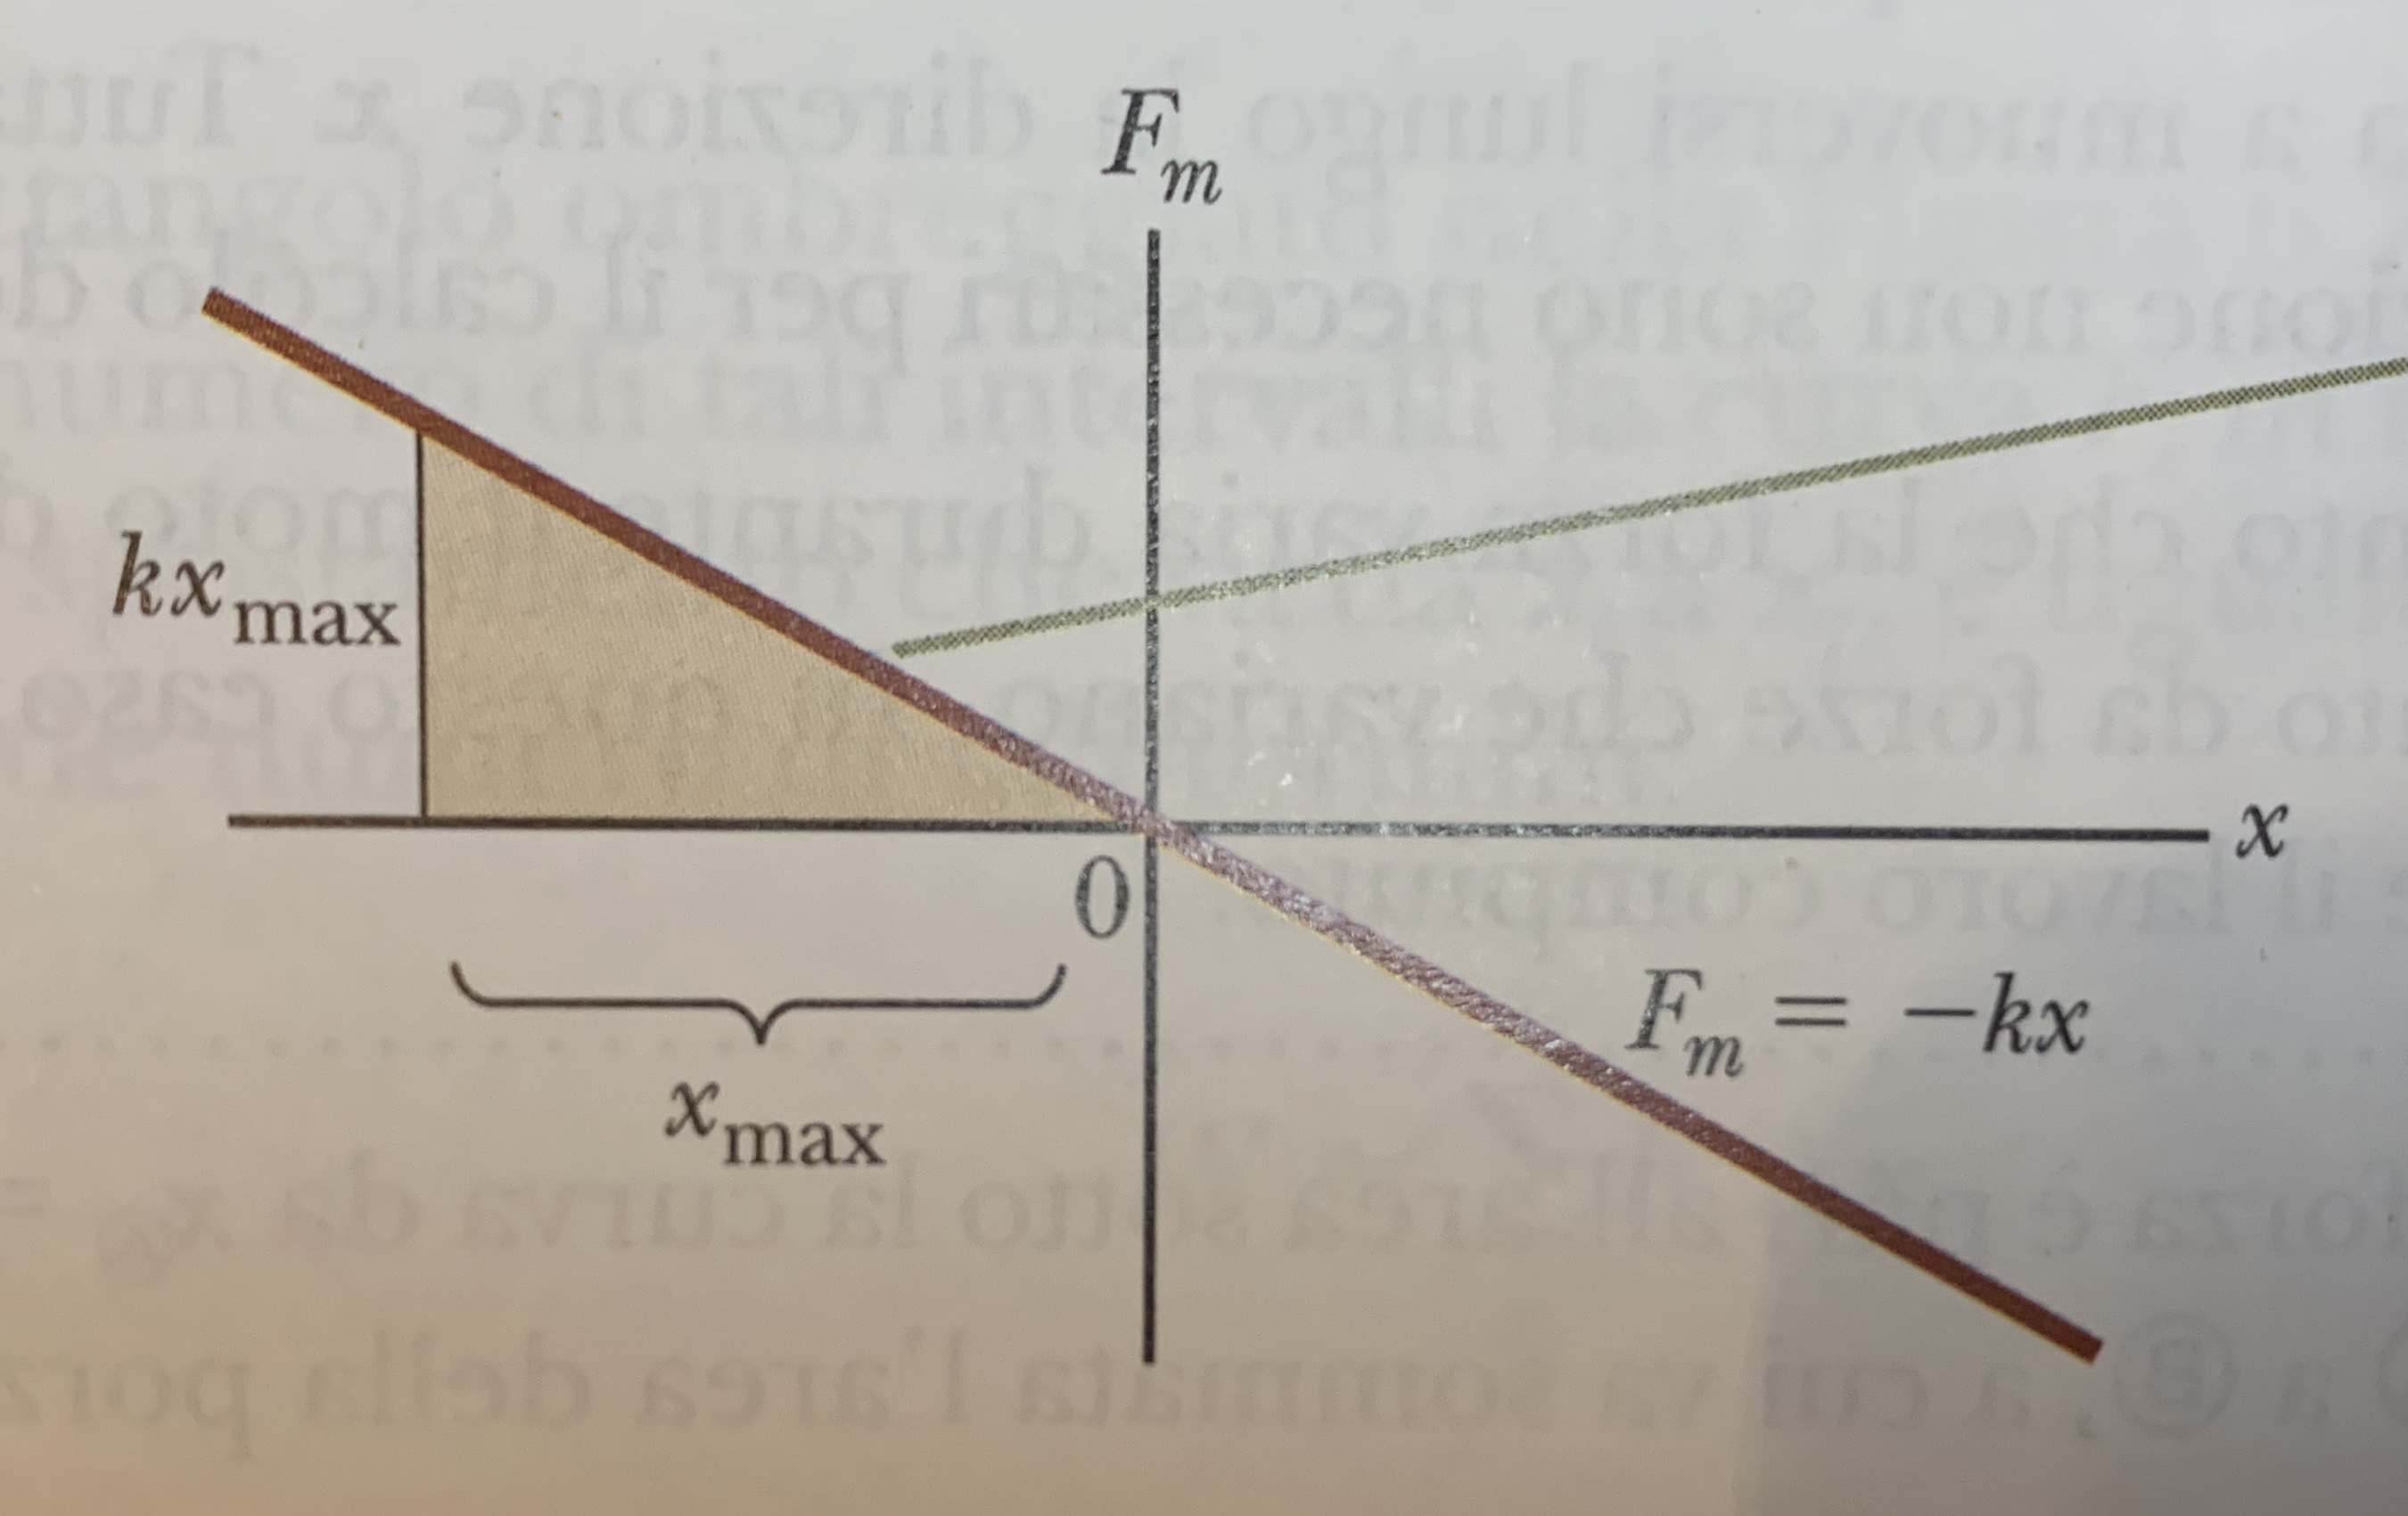
\includegraphics[width=0.5\textwidth]{IMG_2434.jpg}
        \caption{Il lavoro corrisponde all'area del triangolo, quindi $W=-{1 \over 2}kx^2$}
    \end{figure}
    \FloatBarrier
    Se il blocco compie uno spostamento arbitrario da $x_i$ a $x_f$ allora il lavoro sarà dato da
    $$W_{est} = \int_{x_i}^{x_f} kx \ dx = {1 \over 2} kx_f^2 - {1 \over 2} kx_i^2$$
    \newpage
    \subsection{Forze conservative}
    Una forza è detta \textbf{conservativa} se:
    \begin{itemize}
        \item Il \textbf{lavoro totale} che compie \textbf{su una particella} è \textbf{NULLO}
        \item Il \textbf{lavoro} compiuto su una particella cge si muove tra due punti qualsiasi \textbf{non dipende dal percorso seguito}
    \end{itemize}
    \subsection{Energia potenziale}
    Con energia potenziale ci si riferisce all'energia \textbf{associata alla disposizione di due o più corpi} (configurazione di un sistema)
    $$\Delta U = -L$$
    \textbf{Ad ogni forza conservativa è associata un'energia potenziale}
    \subsubsection{Energia potenziale gravitazionale}
    Consideriamo uno spostamento verticale $\Delta y = y_f - y_i$
    \begin{itemize}
        \item $\Delta U = -L = -(F_g \cdot \Delta y \cdot cos\ang{90}) = F_g \cdot \Delta y = mg \cdot \Delta y$  
        \item Cosiderando $y_i=0 \rightarrow \Delta U = mgh$ 
    \end{itemize}
    \subsubsection{Energia potenziale elastica}
    $$\Delta U = -L \rightarrow \Delta U = -(-{1 \over 2}kx^2) \rightarrow \Delta U = {1 \over 2}kx^2$$
    \newpage
    \subsection{Principio di conservazione dell'energia meccanica}
    \paragraph{} L'\textbf{energia meccanica} è definita come $$E = U + K$$
    \paragraph{} Da questa equazione otteniamo che $$\Delta E = \Delta U + \Delta K$$
    $$\Delta E = - L + L = 0$$
    Di conseguenza \begin{itemize}
        \item $\Delta E = 0$ per delle \textbf{forze conservative}
        \item $\Delta E = L_{forze non cons}$ per delle \textbf{forze non conservative}
    \end{itemize}
    In pratica si possono mettere in relazione energia cinetica ed energia potenziale \textbf{senza aver bisogno di conoscere gli stati intermedi}
    \newpage
    \subsection{Curva dell'energia potenziale}
    Data la definizione di energia potenziale, è possibile trovare la definizione analitica della forza $F$
    $$\Delta U (x) = -F(x)\cdot \Delta x$$
    $$F(x) = - {\Delta U (x) \over \Delta x}$$
    $$\lim_{x\to 0} {- {\Delta U (x) \over \Delta x}} = {-{dU(x) \over dx}}$$
    Viene data una curva $U(x)$ che rappresenta la variazione di energia potenziale in relazione allo spostamento e una retta $y = 5 J$ che rappresenta l'energia meccanica in relazione allo spostamento
    \FloatBarrier
    \begin{figure}[!htb]
        \centering
        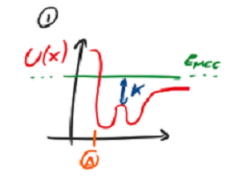
\includegraphics[width=0.5\textwidth]{graph1.PNG}
    \end{figure}
    \FloatBarrier
    Posso trovare $K(x)$ facendo $E_m - U(x)$
    \FloatBarrier
    \begin{figure}[!htb]
        \centering
        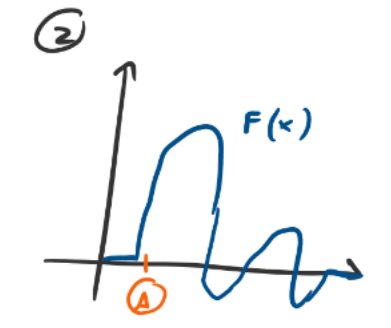
\includegraphics[width=0.5\textwidth]{graph2.PNG}
    \end{figure}
    \FloatBarrier
    Posso trovare $F(x)$ derivando $U(x)$ e ruotandola rispetto all'asse $x$ come da definizione precedente
    \paragraph{} I punti in cui $K=0$ sono detti \textbf{punti di inversione}, dove il corpo si accinge a cambiare direzione. I punti di inversione \textit{possono creare situazioni di \textbf{equilibrio}}:
    \begin{itemize}
        \item \textbf{Equilibrio indifferente}: per ogni punto in cui $E_m = U(x)$ la particella è \textbf{ferma} e può andare sia a sinistra che a destra con la stessa facilità
        \FloatBarrier
        \begin{figure}[!htb]
            \centering
            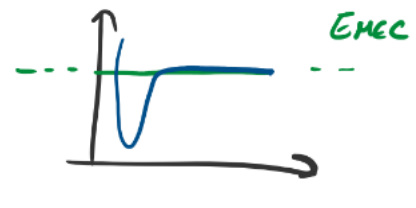
\includegraphics[width=0.5\textwidth]{graph3.PNG}
        \end{figure}
        \FloatBarrier
        \item \textbf{Equilibrio instabile}: la particella è \textbf{ferma}, ma con una \textbf{minima variazione di forza} può muoversi a destra o a sinistra
        \FloatBarrier
        \begin{figure}[!htb]
            \centering
            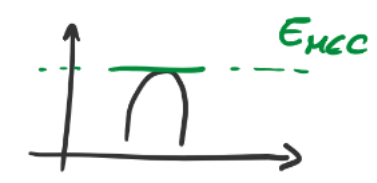
\includegraphics[width=0.5\textwidth]{graph4.PNG}
        \end{figure}
        \FloatBarrier
        \item \textbf{Equilibrio stabile}: la particella è \textbf{ferma e non si può muovere} in quanto $K(x)$ sarebbe \textit{negativa}
        \FloatBarrier
        \begin{figure}[!htb]
            \centering
            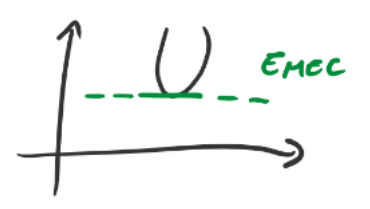
\includegraphics[width=0.5\textwidth]{graph5.PNG}
        \end{figure}
        \FloatBarrier
    \end{itemize}
    \subsection{Conservazione dell'energia}
    In un \textbf{sistema isolato} l'energia interna non può cambiare
    $$\Delta E_m = \Delta E_{th} + \Delta E_{int} = 0$$
    \textbf{In un sistema isolato L = 0}
\end{document}